The knowledge of a mobile robot's initial pose is a prerequisite in tasks
involving its navigation, especially in contexts where an observer is used for
pose tracking. However, the robot's pose is not predictable or pre-settable in
all conditions. This lack of predictability necessitates ad hoc estimation
without prior information. Various sensor and map modalities have been
investigated in the literature; from 2D and 3D LIDAR sensors
\cite{als_eth,Cop2018a}, RGBD cameras \cite{Guo2016}, and RFID equipment
\cite{Tzitzis2023b}, to keyframe-based submaps \cite{Lowry2016} and metric maps
\cite{Rosen2021}. In practice the latter combined with 2D LIDAR sensors have
become the de facto means of mobile robot localisation and navigation due to
the sensor's high measurement precision and frequency, almost no need for
preprocessing, and low cost compared to 3D LIDAR sensors.

This article addresses the problem of Passive Global Localisation of a 2D LIDAR
sensor in a 2D metric map, i.e. the estimation of its location and orientation
within the map, under complete locational and orientational uncertainty,
without prescribing robot motion commands
for further knowledge acquisition. The problem is
formalised in Problem \ref{prob:the_problem}:

%%%%%%%%%%%%%%%%%%%%%%%%%%%%%%%%%%%%%%%%%%%%%%%%%%%%%%%%%%%%%%%%%%%%%%%%%%%%%%%%
\begin{customprb}{P}
  \label{prob:the_problem}
  Let the unknown pose of an immobile 2D range sensor whose angular range is
  $\lambda$ be $\bm{p}(\bm{l},\theta)$, $\bm{l} = (x,y)$, with respect to the
  reference frame of map $\bm{M}$. Let the range sensor measure range scan
  $\mathcal{S}_R$. The objective is the estimation of $\bm{p}$ given
  $\mathcal{S}_R$, $\bm{M}$, and $\lambda$.
\end{customprb}
%%%%%%%%%%%%%%%%%%%%%%%%%%%%%%%%%%%%%%%%%%%%%%%%%%%%%%%%%%%%%%%%%%%%%%%%%%%%%%%%

\begin{figure}\vspace{0.4em}
  % GNUPLOT: LaTeX picture with Postscript
\begingroup
  \makeatletter
  \providecommand\color[2][]{%
    \GenericError{(gnuplot) \space\space\space\@spaces}{%
      Package color not loaded in conjunction with
      terminal option `colourtext'%
    }{See the gnuplot documentation for explanation.%
    }{Either use 'blacktext' in gnuplot or load the package
      color.sty in LaTeX.}%
    \renewcommand\color[2][]{}%
  }%
  \providecommand\includegraphics[2][]{%
    \GenericError{(gnuplot) \space\space\space\@spaces}{%
      Package graphicx or graphics not loaded%
    }{See the gnuplot documentation for explanation.%
    }{The gnuplot epslatex terminal needs graphicx.sty or graphics.sty.}%
    \renewcommand\includegraphics[2][]{}%
  }%
  \providecommand\rotatebox[2]{#2}%
  \@ifundefined{ifGPcolor}{%
    \newif\ifGPcolor
    \GPcolorfalse
  }{}%
  \@ifundefined{ifGPblacktext}{%
    \newif\ifGPblacktext
    \GPblacktexttrue
  }{}%
  % define a \g@addto@macro without @ in the name:
  \let\gplgaddtomacro\g@addto@macro
  % define empty templates for all commands taking text:
  \gdef\gplfronttext{}%
  \gdef\gplfronttext{}%
  \makeatother
  \ifGPblacktext
    % no textcolor at all
    \def\colorrgb#1{}%
    \def\colorgray#1{}%
  \else
    % gray or color?
    \ifGPcolor
      \def\colorrgb#1{\color[rgb]{#1}}%
      \def\colorgray#1{\color[gray]{#1}}%
      \expandafter\def\csname LTw\endcsname{\color{white}}%
      \expandafter\def\csname LTb\endcsname{\color{black}}%
      \expandafter\def\csname LTa\endcsname{\color{black}}%
      \expandafter\def\csname LT0\endcsname{\color[rgb]{1,0,0}}%
      \expandafter\def\csname LT1\endcsname{\color[rgb]{0,1,0}}%
      \expandafter\def\csname LT2\endcsname{\color[rgb]{0,0,1}}%
      \expandafter\def\csname LT3\endcsname{\color[rgb]{1,0,1}}%
      \expandafter\def\csname LT4\endcsname{\color[rgb]{0,1,1}}%
      \expandafter\def\csname LT5\endcsname{\color[rgb]{1,1,0}}%
      \expandafter\def\csname LT6\endcsname{\color[rgb]{0,0,0}}%
      \expandafter\def\csname LT7\endcsname{\color[rgb]{1,0.3,0}}%
      \expandafter\def\csname LT8\endcsname{\color[rgb]{0.5,0.5,0.5}}%
    \else
      % gray
      \def\colorrgb#1{\color{black}}%
      \def\colorgray#1{\color[gray]{#1}}%
      \expandafter\def\csname LTw\endcsname{\color{white}}%
      \expandafter\def\csname LTb\endcsname{\color{black}}%
      \expandafter\def\csname LTa\endcsname{\color{black}}%
      \expandafter\def\csname LT0\endcsname{\color{black}}%
      \expandafter\def\csname LT1\endcsname{\color{black}}%
      \expandafter\def\csname LT2\endcsname{\color{black}}%
      \expandafter\def\csname LT3\endcsname{\color{black}}%
      \expandafter\def\csname LT4\endcsname{\color{black}}%
      \expandafter\def\csname LT5\endcsname{\color{black}}%
      \expandafter\def\csname LT6\endcsname{\color{black}}%
      \expandafter\def\csname LT7\endcsname{\color{black}}%
      \expandafter\def\csname LT8\endcsname{\color{black}}%
    \fi
  \fi
    \setlength{\unitlength}{0.0500bp}%
    \ifx\gptboxheight\undefined%
      \newlength{\gptboxheight}%
      \newlength{\gptboxwidth}%
      \newsavebox{\gptboxtext}%
    \fi%
    \setlength{\fboxrule}{0.5pt}%
    \setlength{\fboxsep}{1pt}%
\begin{picture}(5000.00,3000.00)%
    \gplgaddtomacro\gplfronttext{%
    }%
    \gplgaddtomacro\gplfronttext{%
    }%
    \gplgaddtomacro\gplfronttext{%
    }%
    \gplgaddtomacro\gplfronttext{%
      \colorrgb{0.15,0.15,0.15}%
      \put(475,1279){\makebox(0,0)[r]{\strut{}$0$}}%
      \colorrgb{0.15,0.15,0.15}%
      %\put(791,1256){\makebox(0,0)[r]{\strut{}$5$}}%
      \colorrgb{0.15,0.15,0.15}%
      \put(1107,1233){\makebox(0,0)[r]{\strut{}$10$}}%
      \colorrgb{0.15,0.15,0.15}%
      %\put(1424,1209){\makebox(0,0)[r]{\strut{}$15$}}%
      \colorrgb{0.15,0.15,0.15}%
      \put(1740,1186){\makebox(0,0)[r]{\strut{}$20$}}%
      \colorrgb{0.15,0.15,0.15}%
      %\put(2056,1163){\makebox(0,0)[r]{\strut{}$25$}}%
      \colorrgb{0.15,0.15,0.15}%
      \put(2373,1140){\makebox(0,0)[r]{\strut{}$30$}}%
      \colorrgb{0.15,0.15,0.15}%
      %\put(2688,1117){\makebox(0,0)[r]{\strut{}$35$}}%
      \colorrgb{0.15,0.15,0.15}%
      \put(3004,1094){\makebox(0,0)[r]{\strut{}$40$}}%
      \colorrgb{0.15,0.15,0.15}%
      \put(3528,1236){\makebox(0,0)[l]{\strut{}$0$}}%
      \colorrgb{0.15,0.15,0.15}%
      %\put(3764,1366){\makebox(0,0)[l]{\strut{}$5$}}%
      \colorrgb{0.15,0.15,0.15}%
      \put(4000,1496){\makebox(0,0)[l]{\strut{}$10$}}%
      \colorrgb{0.15,0.15,0.15}%
      %\put(4236,1626){\makebox(0,0)[l]{\strut{}$15$}}%
      \colorrgb{0.15,0.15,0.15}%
      \put(4471,1756){\makebox(0,0)[l]{\strut{}$20$}}%
      \colorrgb{0.15,0.15,0.15}%
      \put(473,2125){\makebox(0,0)[r]{\strut{}$0.0$}}%
      \colorrgb{0.15,0.15,0.15}%
      \put(473,1817){\makebox(0,0)[r]{\strut{}$2.0$}}%
      \colorrgb{0.15,0.15,0.15}%
      \put(473,1509){\makebox(0,0)[r]{\strut{}$4.0$}}%
    }%
    \put(0,0){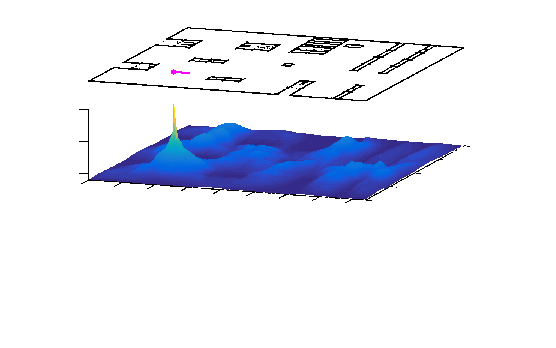
\includegraphics{./figures/face_top}}%
    \gplfronttext
  \end{picture}%
\endgroup

  \vspace{-1.65cm}
  \caption{\small Top: the map of an environment and the pose of a panoramic 2D
           LIDAR sensor (magenta). Given a LIDAR sensor's 2D measurement, at its
           core, CBGL disperses pose hypotheses within the map and ranks them
           ascendingly (bottom) according to the value of the Cumulative
           Absolute Error per Ray metric (Eq. (\ref{eq:caer})). This
           ranking may estimate the pose of the sensor (a) quickly due to the
           metric's low computational complexity, and (b) accurately due to (i)
           proportionality between the pose estimate error and the value of the
           metric for pose estimates in a neighbourhood of the sensor's pose,
           and (ii) lack of disproportionality outside of that neighbourhood
           (Fig. \ref{fig:motivation_caer})
           }
  \label{fig:face}
\end{figure}

For the solution to Problem \ref{prob:the_problem} this article introduces
CBGL: a single-shot Monte Carlo method
(a) which makes no assumptions regarding the structure or the particulars of the
sensor's environment or the sensor's characteristics,
(b) whose pose errors exhibit robustness to varying sensor angular range, and
(c) which operates with three optionally-set and intuitive parameters, which
trade accuracy for execution time.
The central contributions of the article are:
\begin{itemize}
  \item To the best of the author's knowledge the fastest Monte Carlo global
        localisation method that employs a 2D LIDAR that achieves higher
        pose discovery rates than state-of-the-art methods
  \item The extension and validation of the Cumulative Absolute Error per Ray
        metric's ability to estimate pose error hierarchies solely from real
        and virtual range scans, extended from scan--to--map-scan matching
        (\texttt{sm2}) during pose-tracking, where pose estimates are ``few"
        ($\leq$$2^5$) and their errors are ``small", to the context of global
        localisation, where the set of hypotheses and their errors may be
        arbitrarily large
  \item The thorough evaluation of the proposed method against (a) established
        state-of-the-art localisation methods, (b) real and publicly available
        benchmark conditions, and (c) varying characteristics of environments
        and sensors, which target real conditions, that pose hindrances to
        global localisation methods
\end{itemize}

The rest of the article is structured as follows: Section
\ref{section:definitions} provides necessary definitions and the notation
employed. Section \ref{section:sota} gives a brief review of
solutions to problem \ref{prob:the_problem}, and the relation of the proposed
method to them. The latter's methodology is presented in section
\ref{section:the_proposed_method}, its evaluation in section
\ref{section:results}, and its limitations in section
\ref{section:characterisation}. Section \ref{section:finale} concludes this
study.
